\section{Pembahasan Hasil dari Proses}
Pada bab ini saya akan memaparkan dan menjelaskan hasil dari masing-masing proses yang telah kita jalankan baik menggunakan komputer pribadi maupun menggunakan google colab.
\begin{enumerate}
\item Proses pertama yaitu encoder peprocessing, pada proses ini input yang dibutuhkan yaitu file audio dataset dengan struktur folder seperti gambar \ref{hasil2}. Pertama yaitu membuat folder dengan nama dataset, lalu buat folder dengan nama dataset yang digunakan, contoh pada gambar menggunakan dataset titml. Apabila folder dengan nama dataset telah dibuat, maka buat folder dengan nama speaker misalnya f01 (female01), f02 (female02) dan seterusnya untuk speaker dengan jenis kelamin perempuan. Berikan nama folder m01 (male), m02 (male02) dan seterusnya untuk speaker dengan jenis kelamin laki-laki. Isikan file audio sesuai dengan masing-masing folder. Masukkan file suara female01 ke folder f01 dan seterusnya. Hal ini dilakukan agar model dapat mengenali suara setiap speaker pada dataset dan memudahan model dalam mempelajari suara masing-masing speaker, memetakan dan menampilkan hasilnya menggunakan library umap-learn.

\begin{figure}[H]
    \centering
    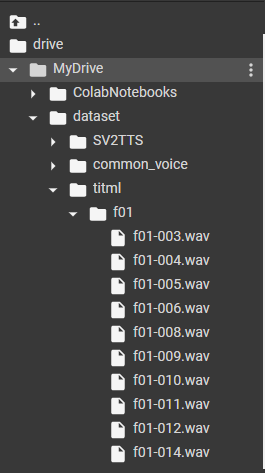
\includegraphics[scale=0.5]{figures/hasil2}
    \caption{\textit{Struktur Folder Dataset untuk Preprocessing Speaker Encoder}}
    \label{hasil2}
\end{figure}

Berikut hasil dari proses encoder preprocessing:
\begin{figure}[H]
    \centering
    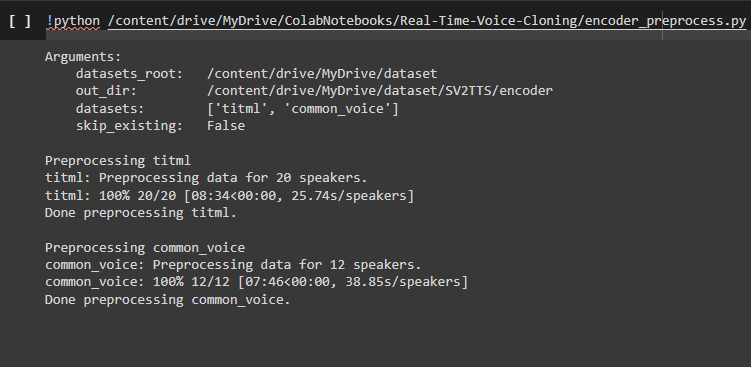
\includegraphics[scale=0.5]{figures/hasil3}
    \caption{\textit{Hasil Preprocessing Speaker Encoder}}
    \label{hasil3}
\end{figure}

Periksa folder dataset lalu buka folder dengan nama SV2TTS, didalam folder tersebut teman-teman akan menemukan folder dengan nama encoder yang didalamnya terdapat hasil preprocessing encoder. Perhatikan gambar \ref{hasil4} terdapat 32 folder yang mewakilkan masing-masing speaker, didalam folder tersebut terdapat numpy array hasil preprocess dari dataset titml dan common\_voice yang saya gunakan.
\begin{figure}[H]
    \centering
    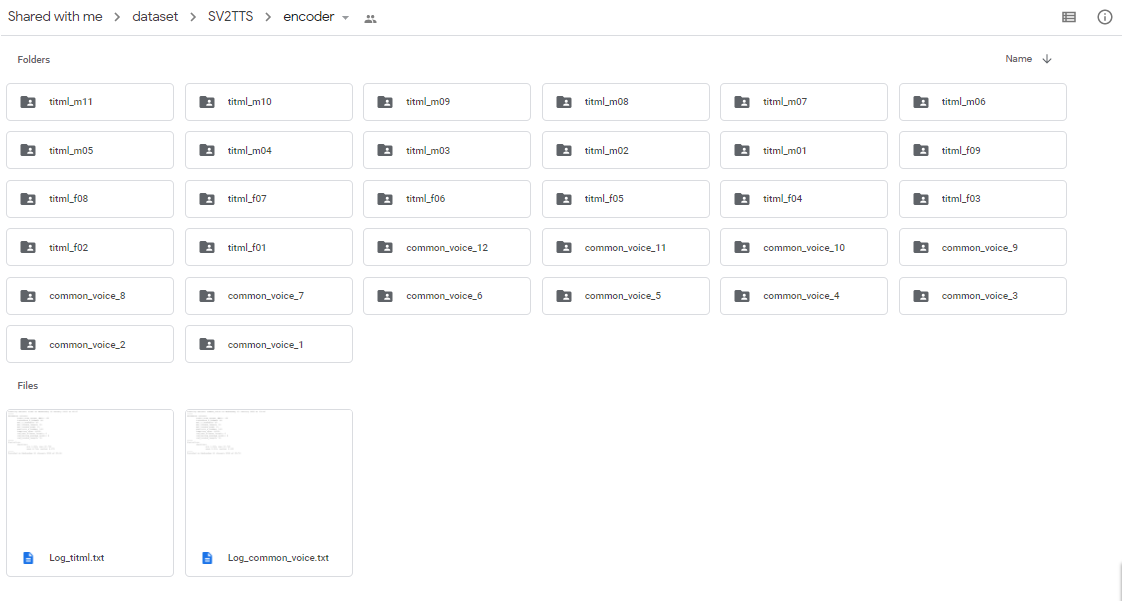
\includegraphics[scale=0.35]{figures/hasil4}
    \caption{\textit{Folder Hasil Preprocessing Speaker Encoder}}
    \label{hasil4}
\end{figure}

\begin{figure}[H]
    \centering
    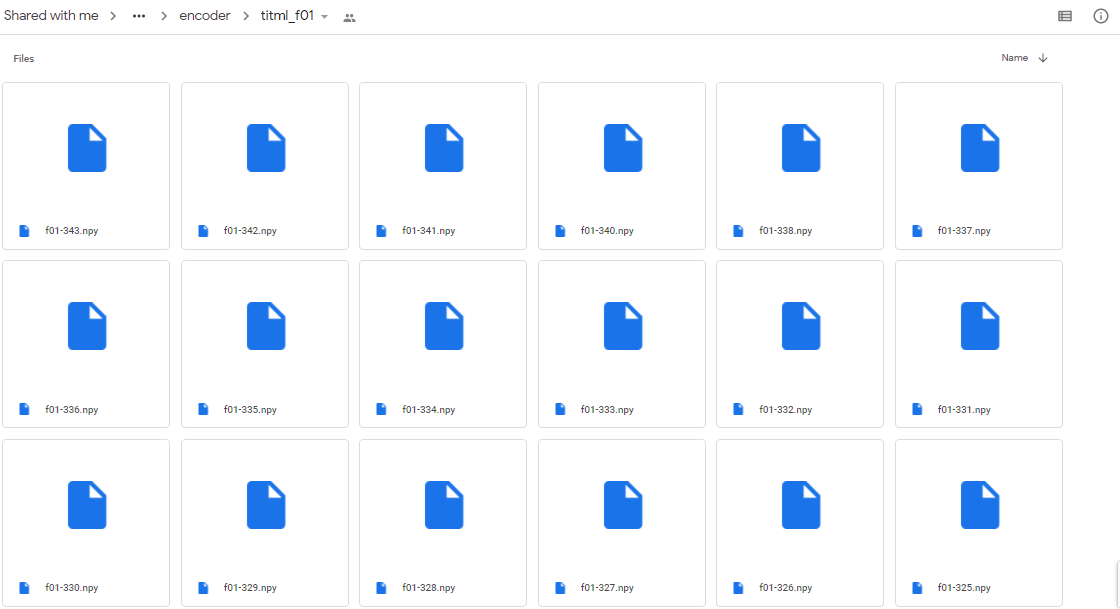
\includegraphics[scale=0.35]{figures/hasil5}
    \caption{\textit{File Numpy Array Hasil Preprocessing Speaker Encoder}}
    \label{hasil5}
\end{figure}

Berikut log hasil preprocessing encoder menggunakan dataset titml dan common\_voice:
\begin{figure}[H]
    \centering
    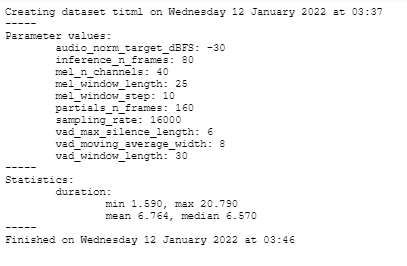
\includegraphics[scale=0.75]{figures/hasil6}
    \caption{\textit{Log TITML-IDN}}
    \label{hasil6}
\end{figure}

\begin{figure}[H]
    \centering
    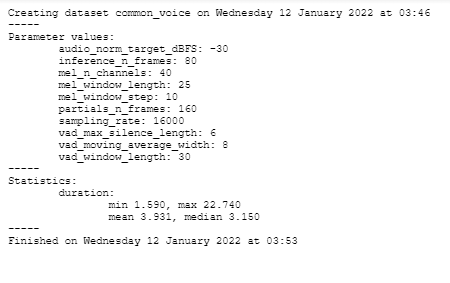
\includegraphics[scale=0.75]{figures/hasil7}
    \caption{\textit{Log Common Voice Indonesia}}
    \label{hasil7}
\end{figure}

\item Proses training speaker encoder model membutuhkan hasil preprocessing encoder yaitu file numpy array dari audio dataset yang telah di preprocess. Perhatikan gambar \ref{hasil8} saya melakukan proses training selama dua minggu menggunakan google colab, saya memperoleh hasil model dengan loss sekitar 0,7 dan error rate sekitar 0.015. Proses training speaker encoder model bisa kita lihat menggunakan visdom server atau teman-teman bisa melihat hasilnya dalam bentuk gambar yang tersimpan di folder pretrained\_backups yang ada di folder Real-Time-Voice-Cloning, masuk ke folder encoder, lalu ke folder saved\_models seperti pada gambar \ref{hasil9}

\begin{figure}[H]
    \centering
    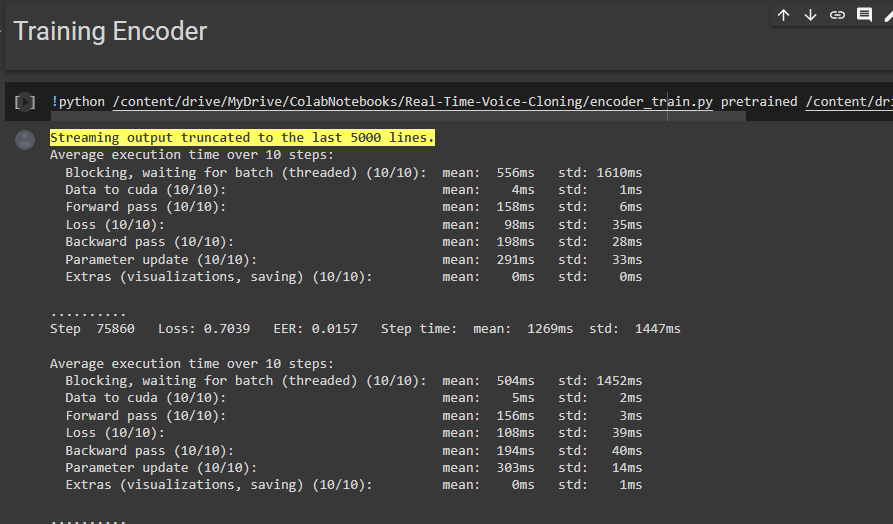
\includegraphics[scale=0.5]{figures/hasil8}
    \caption{\textit{Hasil Training Speaker Encoder Model}}
    \label{hasil8}
\end{figure}

\begin{figure}[H]
    \centering
    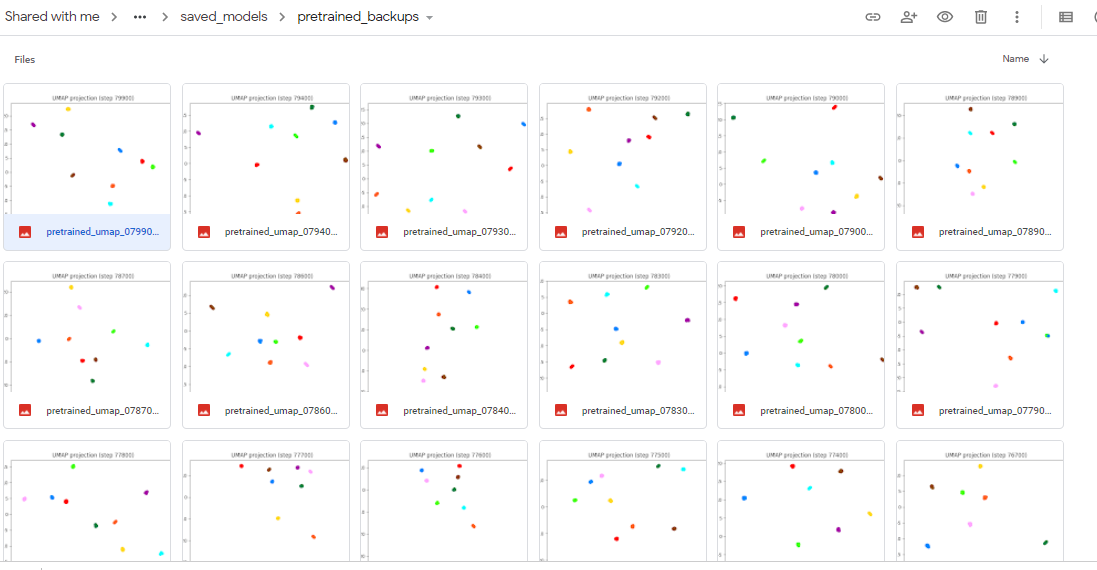
\includegraphics[scale=0.4]{figures/hasil10}
    \caption{\textit{File Hasil Training Speaker Encoder Model}}
    \label{hasil10}
\end{figure}

\begin{figure}[H]
    \centering
    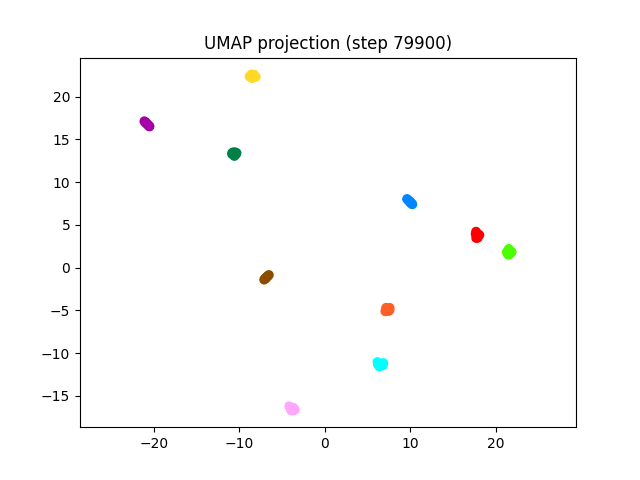
\includegraphics[scale=0.65]{figures/hasil9}
    \caption{\textit{UMAP Projection in 79900 steps}}
    \label{hasil9}
\end{figure}

Berikut hasil dari model yang telah di training dan di save dengan nama file pretrained.pt, file ini akan teman-teman temukan pada folder saved\_models.
\begin{figure}[H]
    \centering
    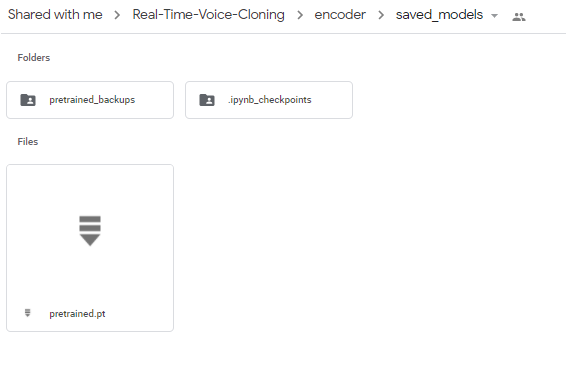
\includegraphics[scale=0.65]{figures/hasil11}
    \caption{\textit{File Speaker Encoder Model}}
    \label{hasil11}
\end{figure}

\item Proses selanjutnya yaitu preprocessing audio, pada tahap ini kita membutuhkan file audio dan file text pada dataset. Dataset yang saya gunakan pada proses ini yaitu common voice indonesia, berikut struktur folder dataset untuk menjalankan preprocessing audio.
\begin{figure}[H]
    \centering
    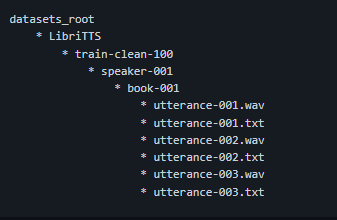
\includegraphics[scale=0.75]{figures/hasil12}
    \caption{\textit{Struktur Dataset untuk Preprocessing Audio dan Embeds}}
    \label{hasil12}
\end{figure}

Proses ini menghasilkan file dengan format numpy array pada folder audio dan mels seperti pada gambar \ref{hasil13}. Selain itu proses ini juga menghasilkan file train.txt yang didalamnya berisi data file name numpy array audio, mels, embeds, serta text dari file audio dataset.

\begin{figure}[H]
    \centering
    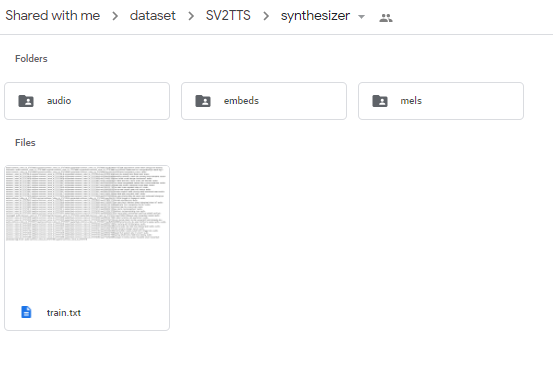
\includegraphics[scale=0.75]{figures/hasil13}
    \caption{\textit{Hasil Preprocessing Audio}}
    \label{hasil13}
\end{figure}

\begin{figure}[H]
    \centering
    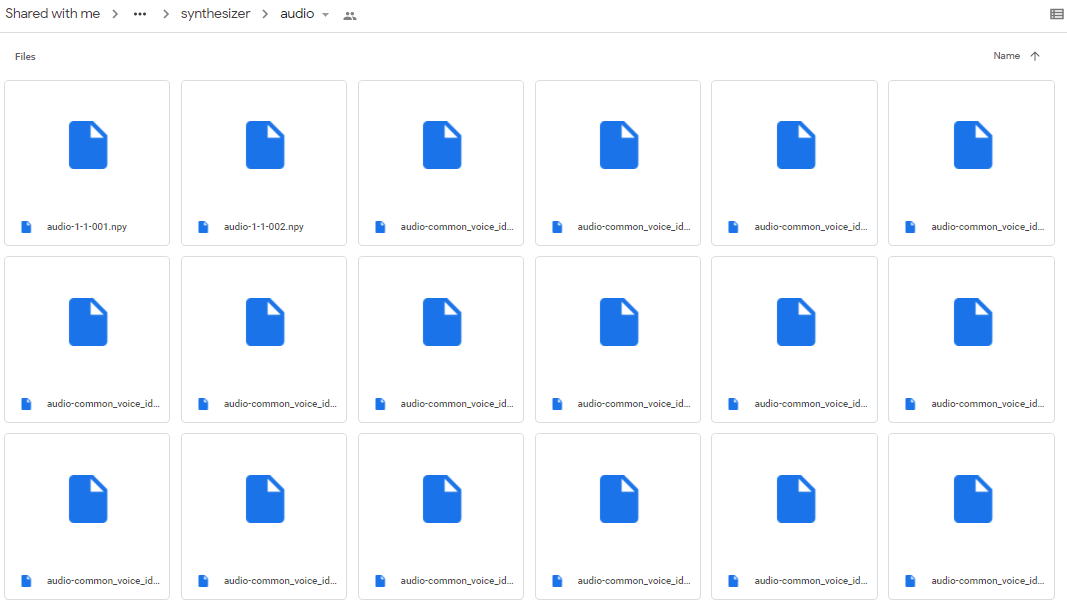
\includegraphics[scale=0.35]{figures/hasil14}
    \caption{\textit{File Numpy Array dari Salah Satu Folder}}
    \label{hasil14}
\end{figure}

\begin{figure}[H]
    \centering
    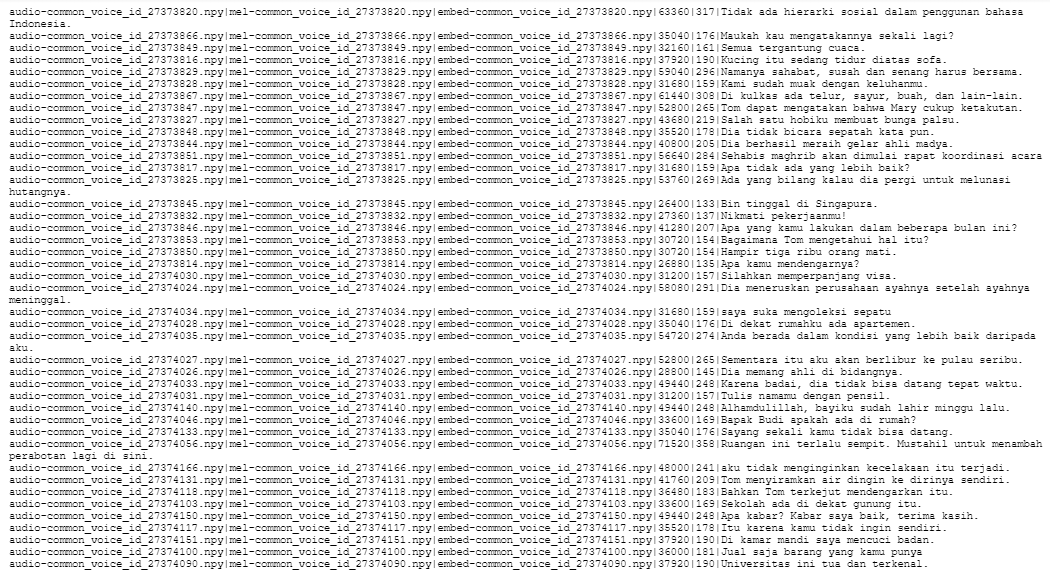
\includegraphics[scale=0.35]{figures/hasil15}
    \caption{\textit{Data Pada File train.txt}}
    \label{hasil15}
\end{figure}

\begin{lstlisting}[caption=Beberapa Data Pada File train.txt]
audio-common_voice_id_27373820.npy|mel-common_voice_id_27373820.npy|embed-common_voice_id_27373820.npy|63360|317|Tidak ada hierarki sosial dalam penggunan bahasa Indonesia.
audio-common_voice_id_27373866.npy|mel-common_voice_id_27373866.npy|embed-common_voice_id_27373866.npy|35040|176|Maukah kau mengatakannya sekali lagi?
audio-common_voice_id_27373849.npy|mel-common_voice_id_27373849.npy|embed-common_voice_id_27373849.npy|32160|161|Semua tergantung cuaca.
audio-common_voice_id_27373816.npy|mel-common_voice_id_27373816.npy|embed-common_voice_id_27373816.npy|37920|190|Kucing itu sedang tidur diatas sofa.
audio-common_voice_id_27373829.npy|mel-common_voice_id_27373829.npy|embed-common_voice_id_27373829.npy|59040|296|Namanya sahabat, susah dan senang harus bersama.
audio-common_voice_id_27373828.npy|mel-common_voice_id_27373828.npy|embed-common_voice_id_27373828.npy|31680|159|Kami sudah muak dengan keluhanmu.
audio-common_voice_id_27373867.npy|mel-common_voice_id_27373867.npy|embed-common_voice_id_27373867.npy|61440|308|Di kulkas ada telur, sayur, buah, dan lain-lain.
audio-common_voice_id_27373847.npy|mel-common_voice_id_27373847.npy|embed-common_voice_id_27373847.npy|52800|265|Tom dapat mengatakan bahwa Mary cukup ketakutan.
audio-common_voice_id_27373827.npy|mel-common_voice_id_27373827.npy|embed-common_voice_id_27373827.npy|43680|219|Salah satu hobiku membuat bunga palsu.
audio-common_voice_id_27373848.npy|mel-common_voice_id_27373848.npy|embed-common_voice_id_27373848.npy|35520|178|Dia tidak bicara sepatah kata pun.
audio-common_voice_id_27373844.npy|mel-common_voice_id_27373844.npy|embed-common_voice_id_27373844.npy|40800|205|Dia berhasil meraih gelar ahli madya.
audio-common_voice_id_27373851.npy|mel-common_voice_id_27373851.npy|embed-common_voice_id_27373851.npy|56640|284|Sehabis maghrib akan dimulai rapat koordinasi acara
audio-common_voice_id_27373817.npy|mel-common_voice_id_27373817.npy|embed-common_voice_id_27373817.npy|31680|159|Apa tidak ada yang lebih baik?
audio-common_voice_id_27373825.npy|mel-common_voice_id_27373825.npy|embed-common_voice_id_27373825.npy|53760|269|Ada yang bilang kalau dia pergi untuk melunasi hutangnya.
\end{lstlisting}

\item Preprocessing Embeds menghasilkan numpy array pada folder embeds yang digenerate berdasarkan pada file train.txt. Berikut hasil preprocessing embeds:
\begin{figure}[H]
    \centering
    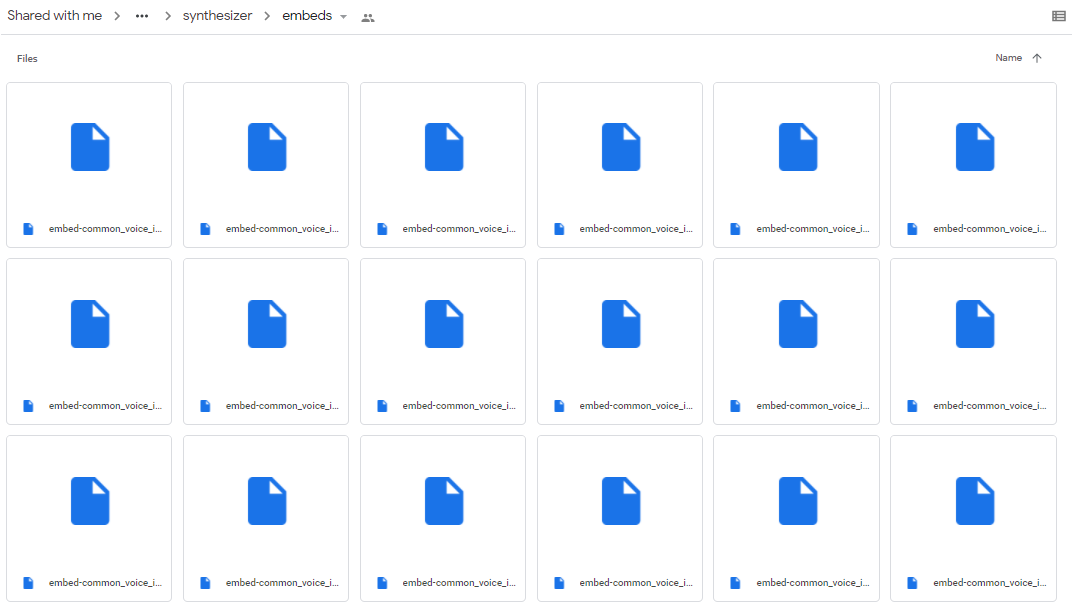
\includegraphics[scale=0.35]{figures/hasil16}
    \caption{\textit{File Numpy Array pada Folder embeds}}
    \label{hasil16}
\end{figure}

\item Proses Training Synthesizer membutuhkan hasil dari preprocessing audio dan preprocessing embeds. Proses training synthesizer menghasilkan prediksi mel-spektrogram terdiri dari 4 folder seperti pada gambar \ref{hasil18}. 
\begin{figure}[H]
    \centering
    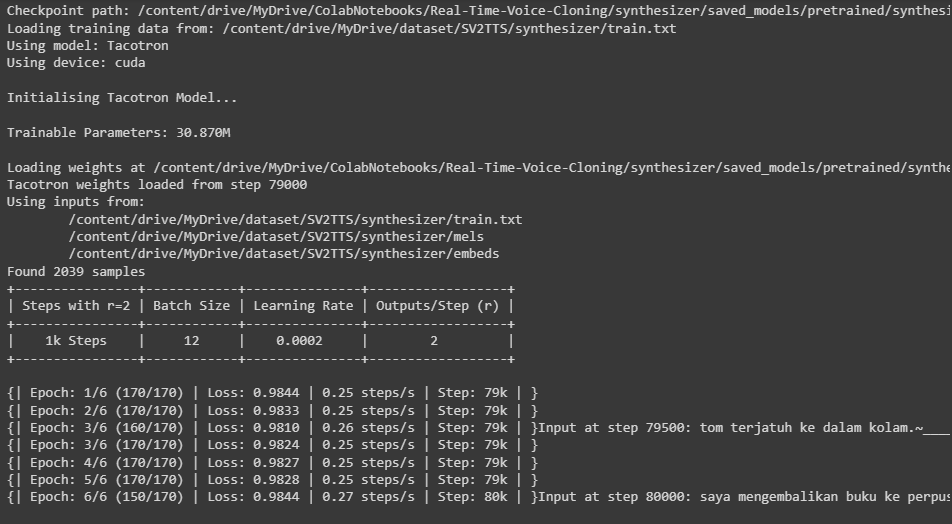
\includegraphics[scale=0.4]{figures/hasil17}
    \caption{\textit{Hasil Proses Training Synthesizer}}
    \label{hasil17}
\end{figure}

\begin{figure}[H]
    \centering
    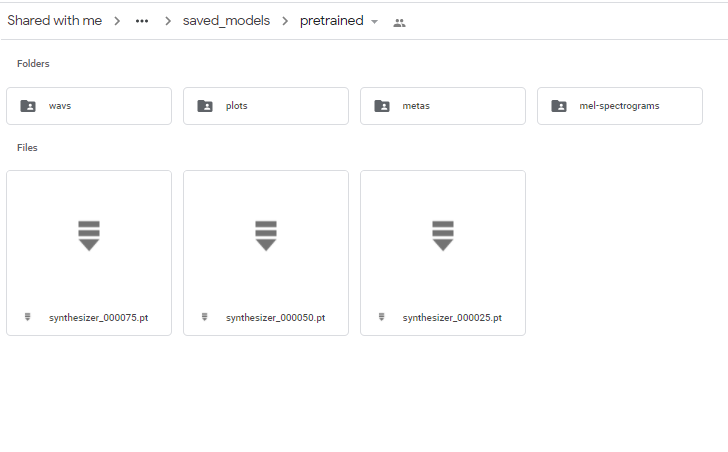
\includegraphics[scale=0.5]{figures/hasil18}
    \caption{\textit{Folder Hasil Proses Training Synthesizer}}
    \label{hasil18}
\end{figure}

Folder wav berisikan file audio prediksi berdasarkan mel-spektrogram seperti pada gambar \ref{hasil19}. 

\begin{figure}[H]
    \centering
    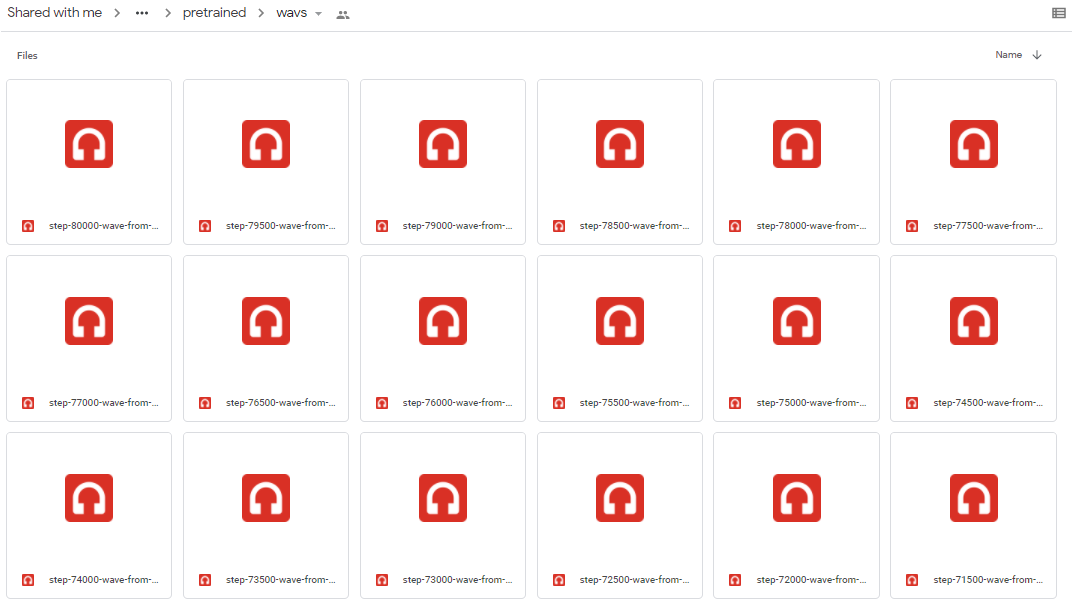
\includegraphics[scale=0.3]{figures/hasil19}
    \caption{\textit{Folder Wav}}
    \label{hasil19}
\end{figure}

Folder plots berisikan visualisasii dari mel-spektrogram seperti pada gambar \ref{hasil20}
\begin{figure}[H]
    \centering
    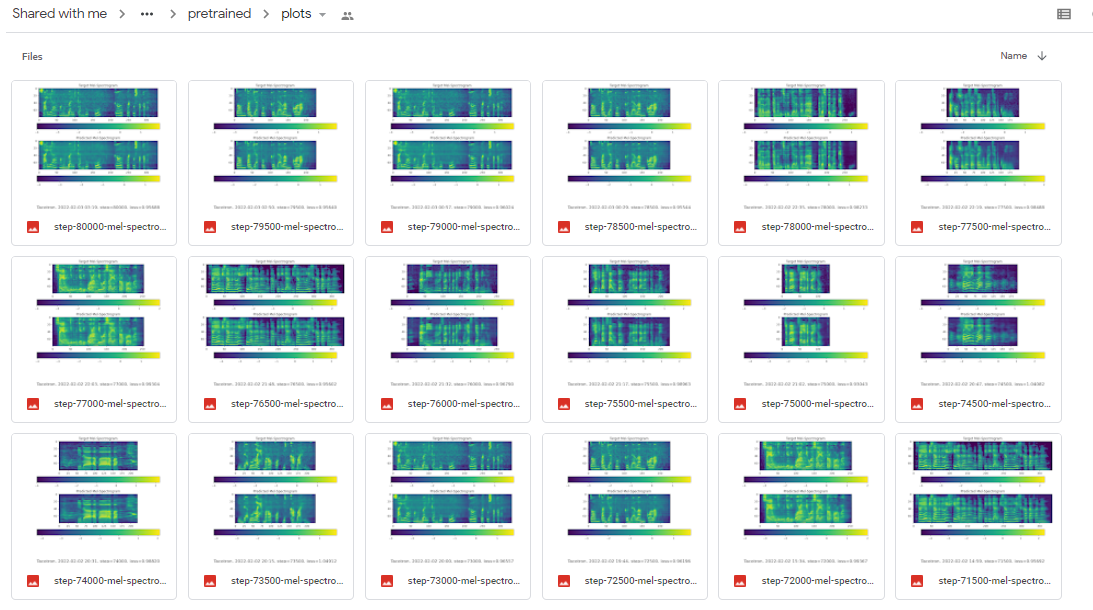
\includegraphics[scale=0.3]{figures/hasil20}
    \caption{\textit{Folder Plots}}
    \label{hasil20}
\end{figure}

 Folder metas berisikan file CharacterEmbeddings.tsv mulai dari a-z hingga angka 0-9 seperti pada gambar \ref{hasil21}.

\begin{figure}[H]
    \centering
    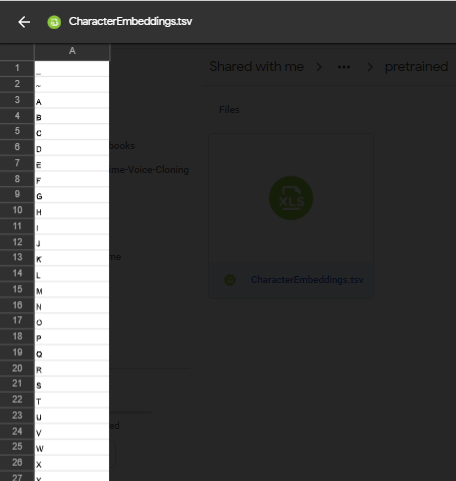
\includegraphics[scale=0.4]{figures/hasil21}
    \caption{\textit{File CharacterEmbeddings.tsv}}
    \label{hasil21}
\end{figure}

Folder mel-spektrogram berisikan file numpy array dari mel-spektrogram seperti pada gambar \ref{hasil22}.

\begin{figure}[H]
    \centering
    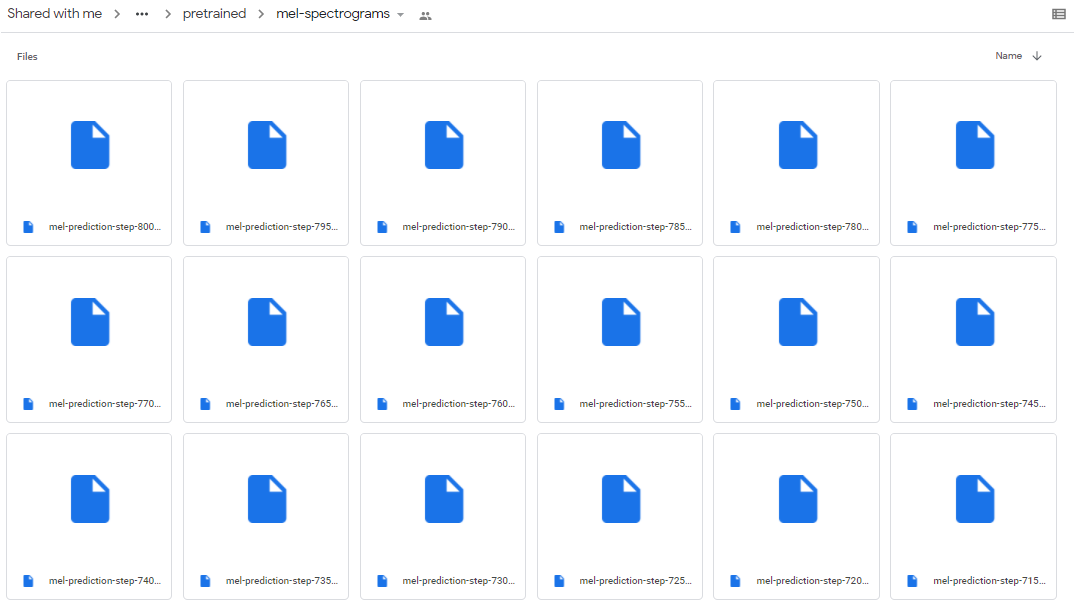
\includegraphics[scale=0.35]{figures/hasil22}
    \caption{\textit{Folder Mel-Spectrogram}}
    \label{hasil22}
\end{figure}

Berikut visualisasi target mel-spectrogram dan predicted mel-spectrogram hasil training synthesizer dengan nilai loss 0.9568.
\begin{figure}[H]
    \centering
    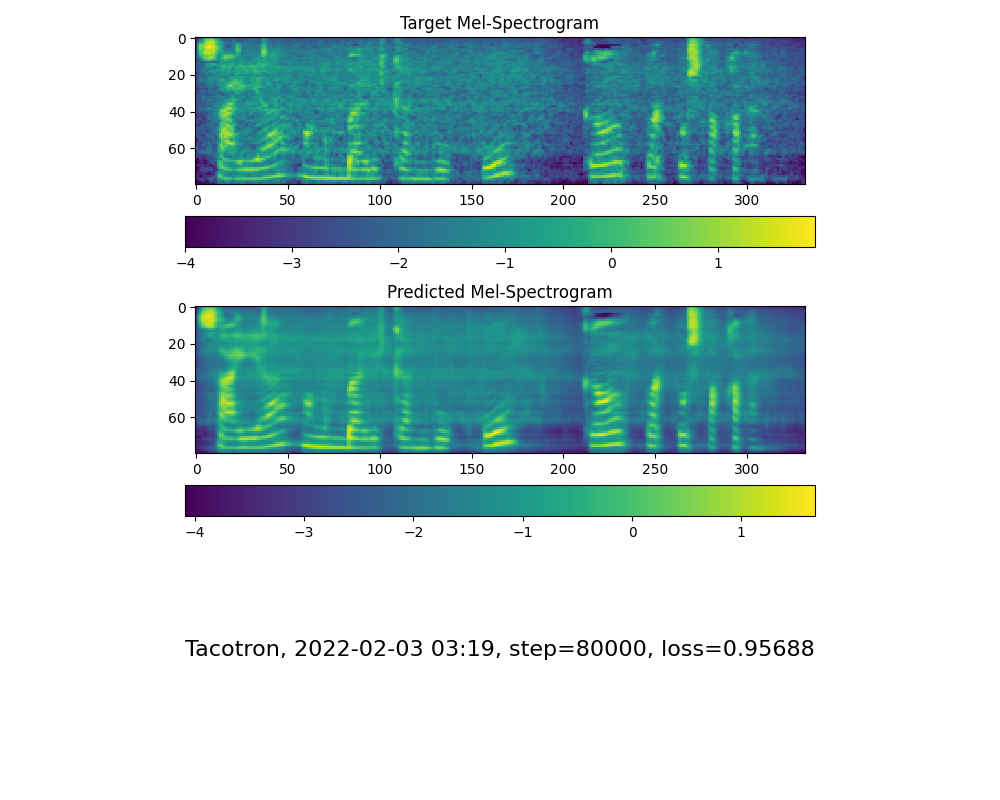
\includegraphics[scale=0.35]{figures/mel}
    \caption{\textit{Mel-Spectrogram}}
    \label{hasil23}
\end{figure}

\item Preprocessing vocoder membutuhkan hasil dari proses training syntesizer model, file train.txt, serta membutuhkan file numpy array mels dan embeds.
\begin{figure}[H]
    \centering
    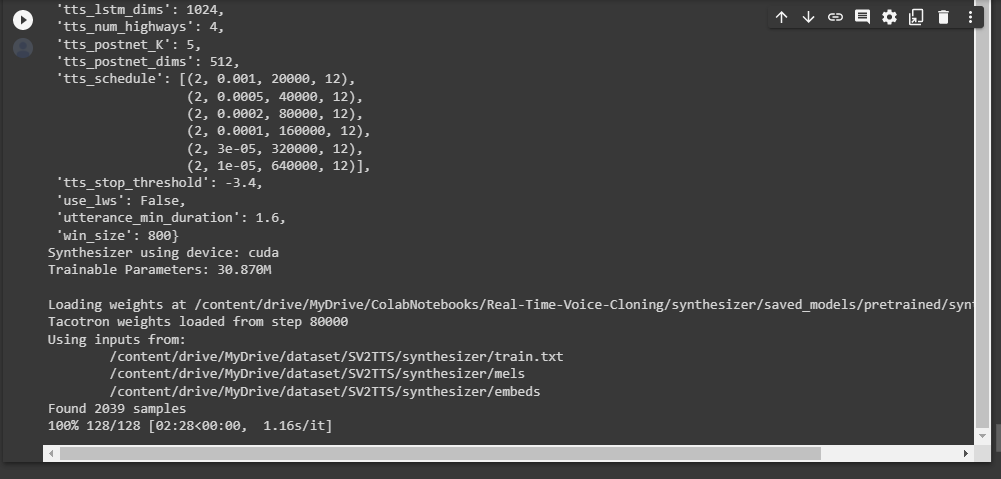
\includegraphics[scale=0.35]{figures/hasil24}
    \caption{\textit{Preprocessing Vocoder}}
    \label{hasil24}
\end{figure}

Proses ini menghasilkan file synthesized.txt dan folder mels-gta yang berisikan file target mel-spectrogram dengan format file binary numpy array yang akan digunakan dalam proses training synthesizer model.
\begin{figure}[H]
    \centering
    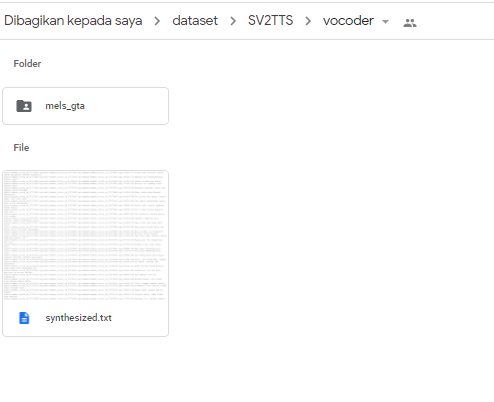
\includegraphics[scale=0.65]{figures/hasil25}
    \caption{\textit{Hasil Preprocessing Vocoder}}
    \label{hasil25}
\end{figure}

\begin{figure}[H]
    \centering
    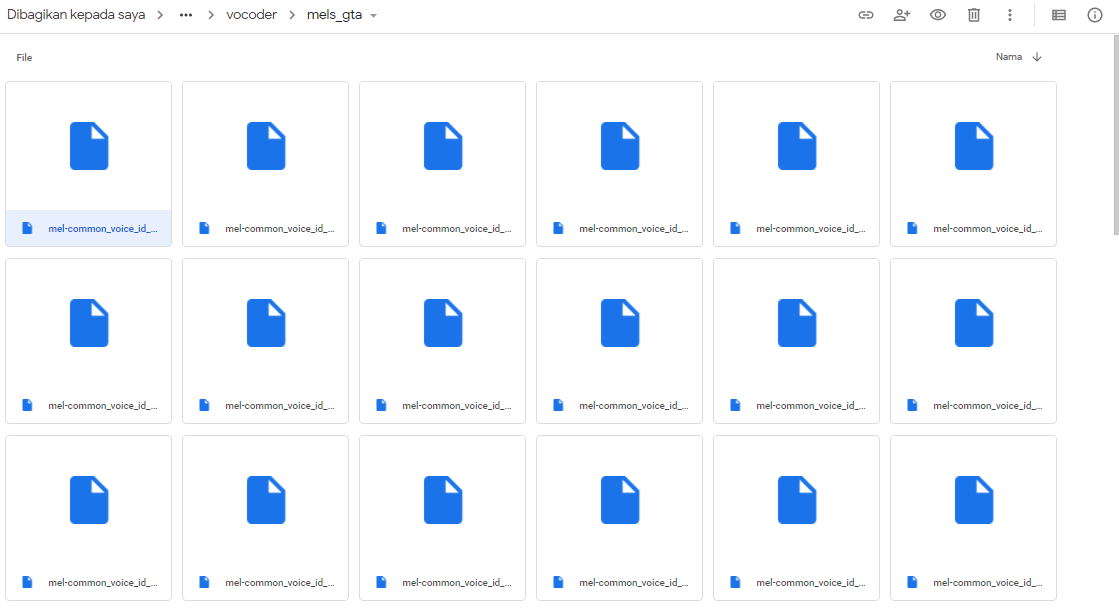
\includegraphics[scale=0.35]{figures/hasil26}
    \caption{\textit{Folder mels-gta}}
    \label{hasil26}
\end{figure}

File synthesized.txt berisikan nama file audio, nama file mel-spectrogram, nama file embeds, dan teks.
\begin{figure}[H]
    \centering
    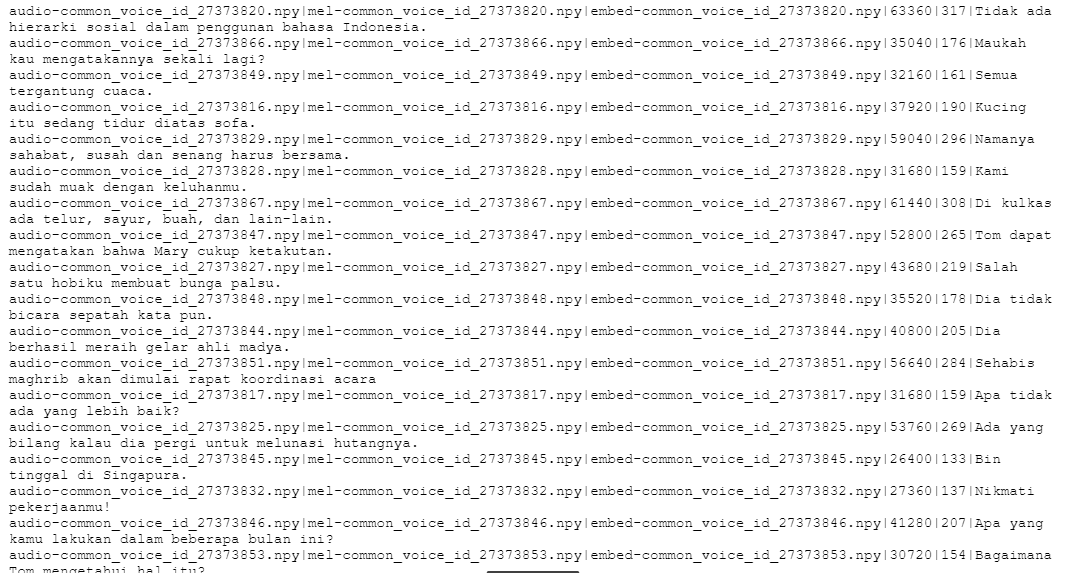
\includegraphics[scale=0.35]{figures/hasil27}
    \caption{\textit{File Synthesized}}
    \label{hasil27}
\end{figure}

\item Proses training vocoder membutuhkan prediksi mel, embeds, target mel, dan file train.txt. Proses ini akan menghasilkan file prediksi audio dari prediksi mel-spectrogram dan menghasilkan target audio dari target mel-spectrogram. Proses generate audio bisa dilihat pada gambar \ref{hasil28}.
\begin{figure}[H]
    \centering
    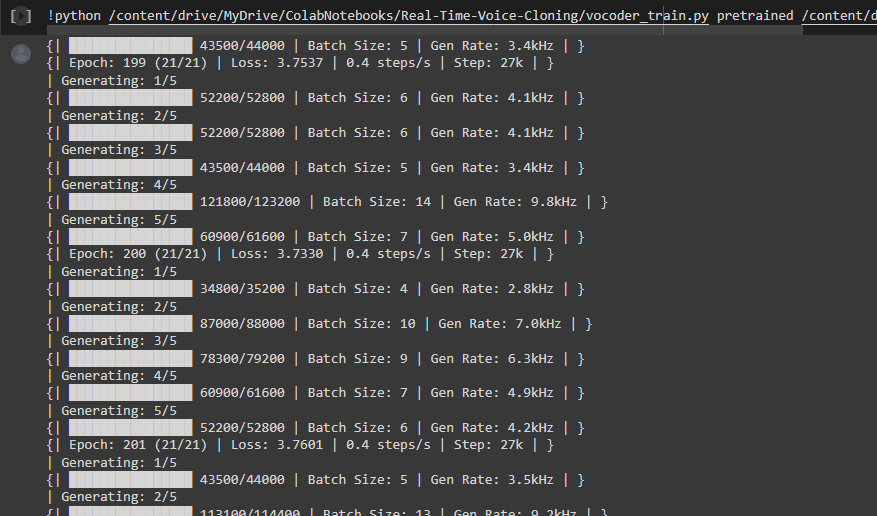
\includegraphics[scale=0.4]{figures/hasil28}
    \caption{\textit{Training Vocoder}}
    \label{hasil28}
\end{figure}

Hasil generate prediksi audio dan target audio bisa teman-teman lihat pada folder saved\_models yang terdapat didalam folder vocoder. Prediksi audio dan target audio bisa teman-teman dengarkan dan menilai hasilnya apakah prediksi audio sudah mendekati target audionya atau belum serta menilai seberapa alami dan kemiripan antara prediksi dan targetnya.
\begin{figure}[H]
    \centering
    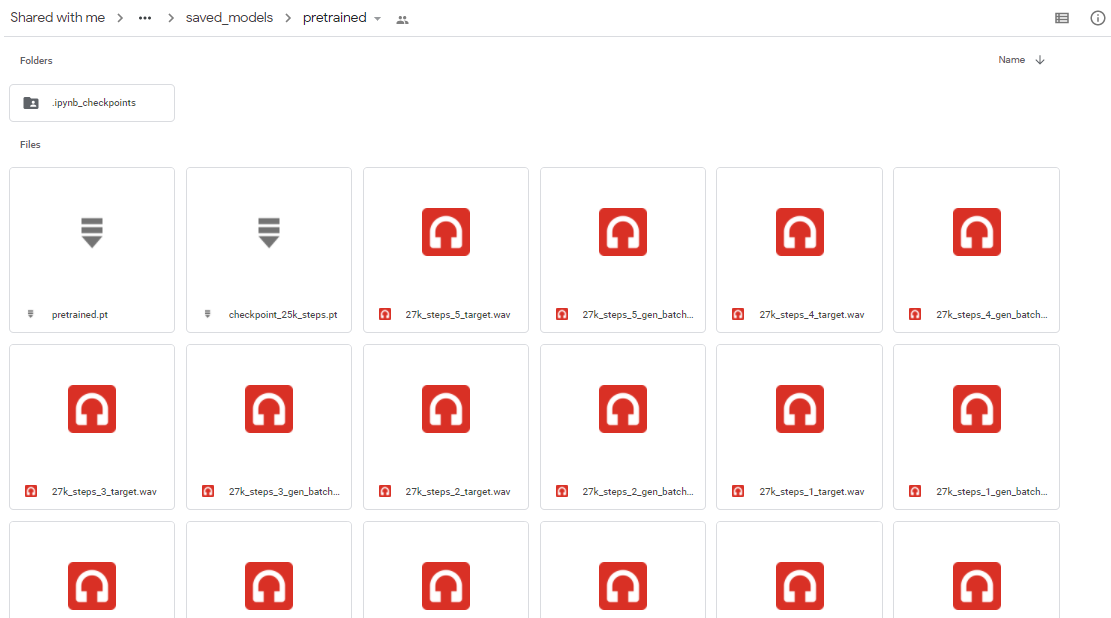
\includegraphics[scale=0.35]{figures/hasil29}
    \caption{\textit{Hasil Generate Audio}}
    \label{hasil29}
\end{figure}

\end{enumerate}

\section{Demo Aplikasi Voice Cloning}
Sekarang kita memiliki tiga model yang telah di training yaitu speaker encoder model, synthesizer model, dan vocoder model. Berikut cara menjalankan aplikasi voice cloning dengan menggunakan ketiga model tersebut.

\begin{enumerate}

\item Pertama buat folder pada google drive dengan nama models, lalu upload ketiga model kedalam folder tersebut seperti pada gambar \ref{tutor2}
\begin{figure}[H]
    \centering
    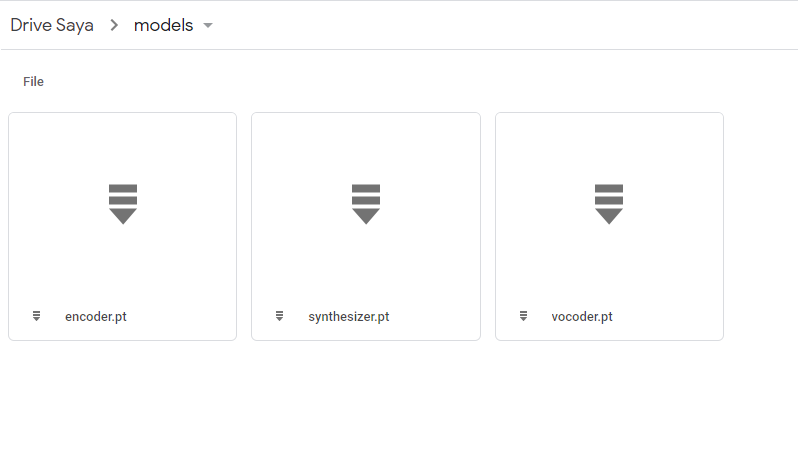
\includegraphics[scale=0.35]{figures/tutor2}
    \caption{\textit{Folder Models}}
    \label{tutor2}
\end{figure}

\item Klik kanan pada file model lalu pilih dapatkan link, ubah akses ke siapa saja yang memiliki link, lalu salin link.

\begin{figure}[H]
    \centering
    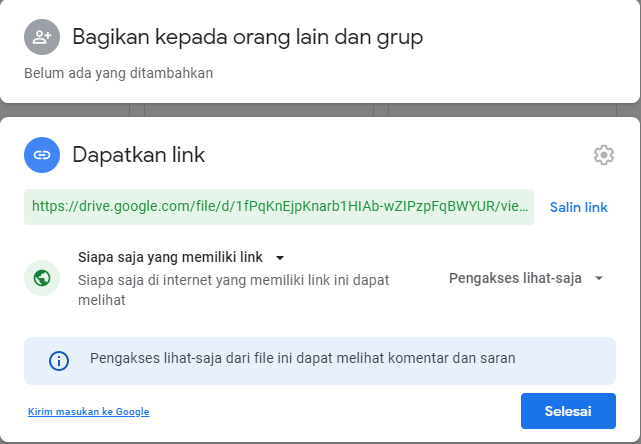
\includegraphics[scale=0.35]{figures/tutor3}
    \caption{\textit{Link Akses}}
    \label{tutor3}
\end{figure}

\item Akses link tersebut dan klik tombol download pada kanan atas, maka link akan berubah menjadi link download seperti berikut \url{https://drive.google.com/u/0/uc?id=1fPqKnEjpKnarb1HIAb-wZIPzpFqBWYUR}. Copy link dan simpan, link ini akan berguna untuk mendownload model teman-teman nantinya. Lakukan hal yang sama pada kedua model lainnya.

\begin{figure}[H]
    \centering
    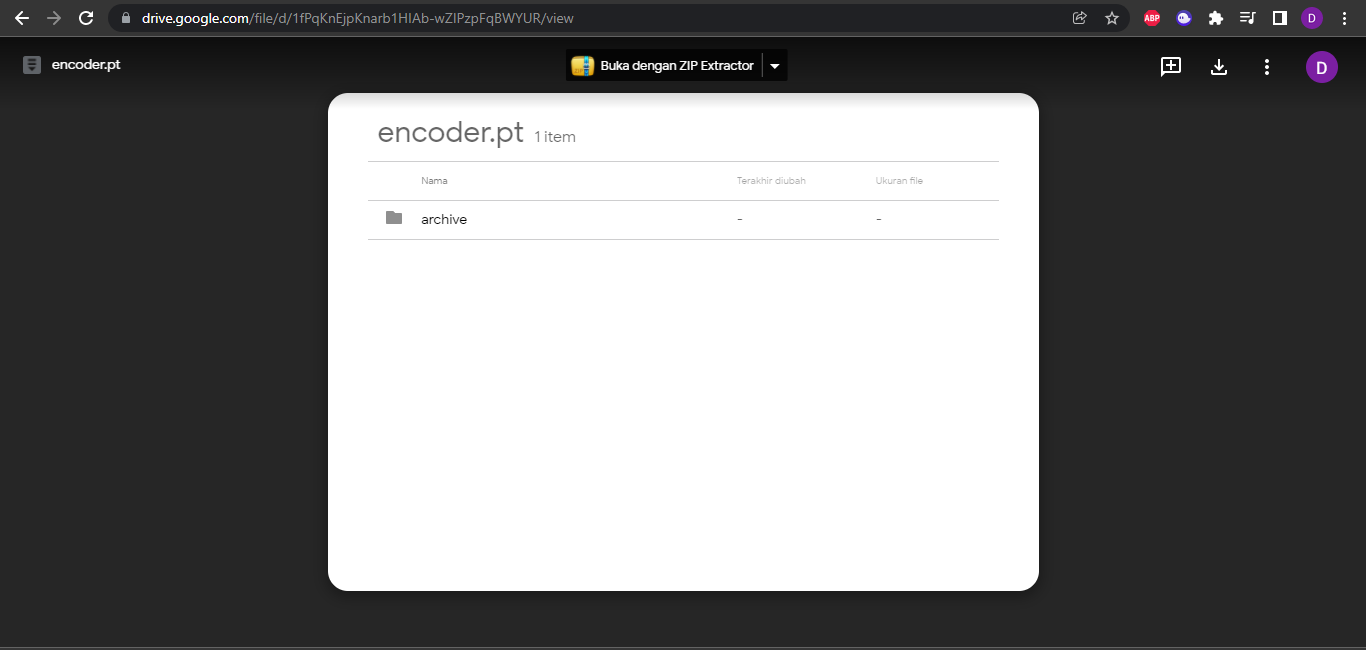
\includegraphics[scale=0.35]{figures/tutor4}
    \caption{\textit{Link Akses}}
    \label{tutor4}
\end{figure}


\item Buat new notebook lalu rename manjadi demo.ipynb. Kemudian tambahkan kode program untuk clone repo, install requirements, dan download model. Paste link download model yang telah teman-teman simpan sebelumnya pada bagian kode program download model.

\begin{figure}[H]
    \centering
    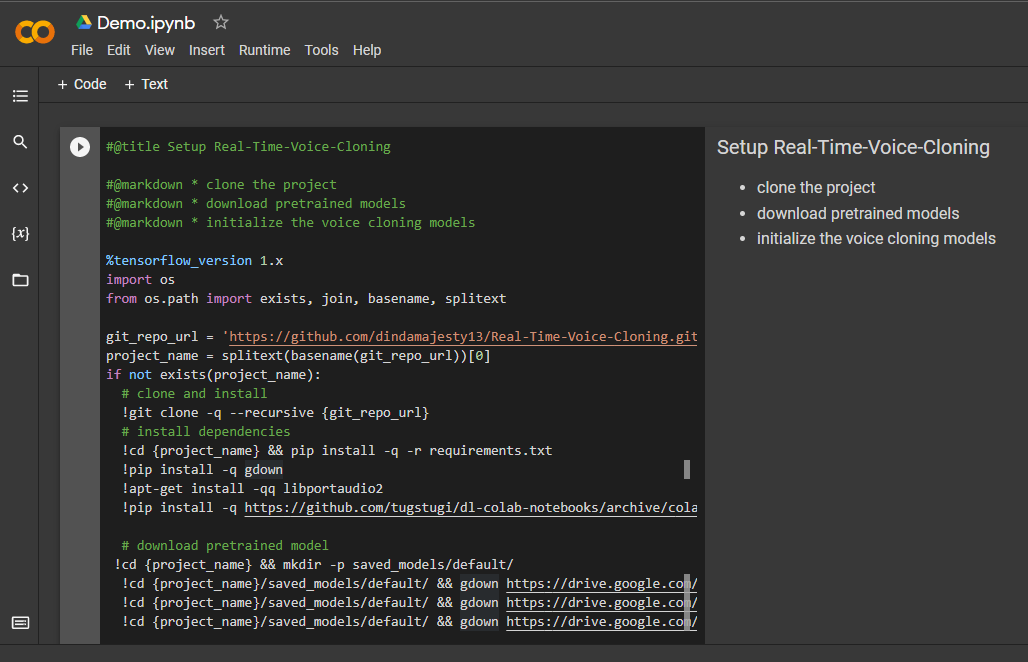
\includegraphics[scale=0.35]{figures/tutor1}
    \caption{\textit{Demo Notebook}}
    \label{tutor1}
\end{figure}

\begin{lstlisting}[language=Python, caption=Setup Project]
#@title Setup CorentinJ/Real-Time-Voice-Cloning

#@markdown * clone the project
#@markdown * download pretrained models
#@markdown * initialize the voice cloning models

%tensorflow_version 1.x
import os
from os.path import exists, join, basename, splitext

#sesuaikan repo dengan repo masing-masing.
git_repo_url = 'https://github.com/dindamajesty13/Real-Time-Voice-Cloning.git'
project_name = splitext(basename(git_repo_url))[0]
if not exists(project_name):
  # clone and install
  !git clone -q --recursive {git_repo_url}
  # install dependencies
  !cd {project_name} && pip install -q -r requirements.txt
  !pip install -q gdown
  !apt-get install -qq libportaudio2
  !pip install -q https://github.com/tugstugi/dl-colab-notebooks/archive/colab_utils.zip

  # download pretrained model
  !cd {project_name} && mkdir -p saved_models/default/
  #paste kan link download model pada kode program di bawah ini.
  !cd {project_name}/saved_models/default/ && gdown https://drive.google.com/uc?id=1fPqKnEjpKnarb1HIAb-wZIPzpFqBWYUR
  !cd {project_name}/saved_models/default/ && gdown https://drive.google.com/uc?id=12oq_PFdcBKsx4BVdSEiSdvg5x5Cyrjza
  !cd {project_name}/saved_models/default/ && gdown https://drive.google.com/uc?id=1_0EHrkS7u1NzQ0WQjeWVdrUYhgOYxQng

import sys
sys.path.append(project_name)

from IPython.display import display, Audio, clear_output
from IPython.utils import io
import ipywidgets as widgets
import numpy as np
from dl_colab_notebooks.audio import record_audio, upload_audio

from synthesizer.inference import Synthesizer
from encoder import inference as encoder
from vocoder import inference as vocoder
from pathlib import Path

!ls 
encoder.load_model(project_name / Path("saved_models/default/encoder.pt"))
synthesizer = Synthesizer(project_name / Path("saved_models/default/synthesizer.pt"))
vocoder.load_model(project_name / Path("saved_models/default/vocoder.pt"))
    
\end{lstlisting}

\item Klik tambahkan code lalu ketikkan kode program berikut untuk record atau upload suara sampel.

\begin{figure}[H]
    \centering
    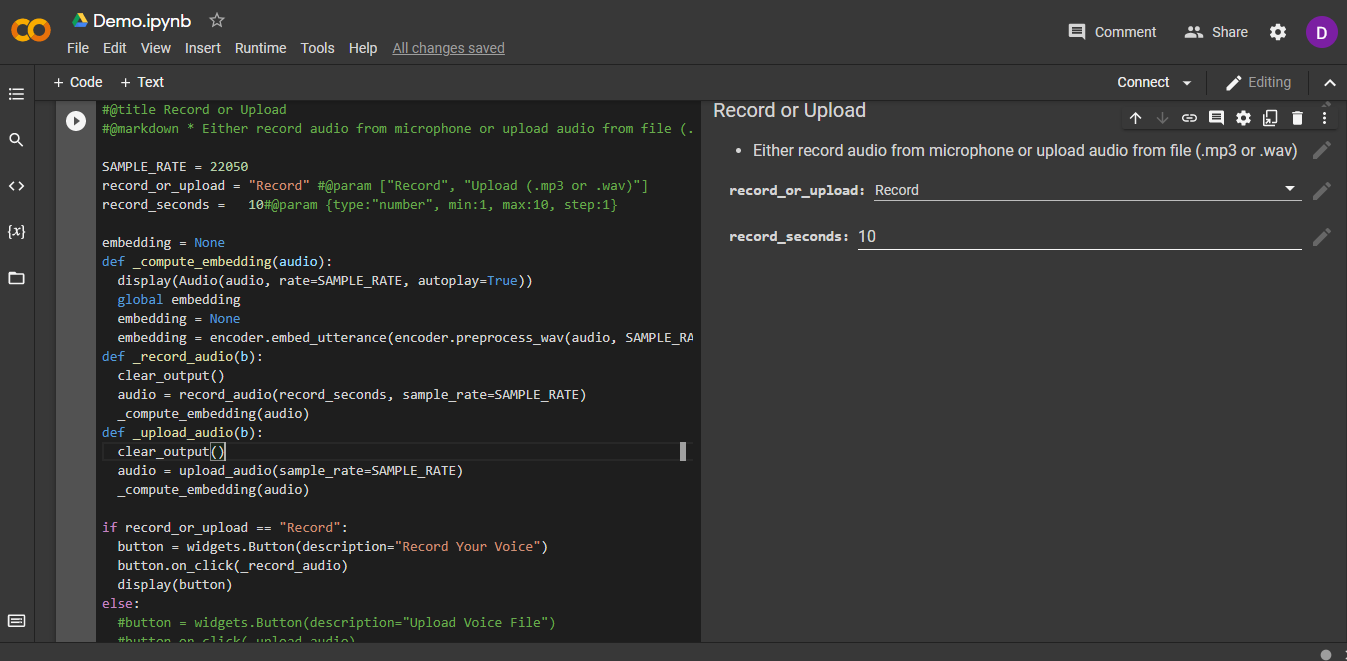
\includegraphics[scale=0.35]{figures/tutor5}
    \caption{\textit{Record or Upload Audio Sample}}
    \label{tutor5}
\end{figure}

\begin{lstlisting}[language=Python, caption=Record or Upload Audio Sample]
#@title Record or Upload
#@markdown * Either record audio from microphone or upload audio from file (.mp3 or .wav) 

SAMPLE_RATE = 22050
record_or_upload = "Record" #@param ["Record", "Upload (.mp3 or .wav)"]
record_seconds =   10#@param {type:"number", min:1, max:10, step:1}

embedding = None
def _compute_embedding(audio):
  display(Audio(audio, rate=SAMPLE_RATE, autoplay=True))
  global embedding
  embedding = None
  embedding = encoder.embed_utterance(encoder.preprocess_wav(audio, SAMPLE_RATE))
def _record_audio(b):
  clear_output()
  audio = record_audio(record_seconds, sample_rate=SAMPLE_RATE)
  _compute_embedding(audio)
def _upload_audio(b):
  clear_output()
  audio = upload_audio(sample_rate=SAMPLE_RATE)
  _compute_embedding(audio)

if record_or_upload == "Record":
  button = widgets.Button(description="Record Your Voice")
  button.on_click(_record_audio)
  display(button)
else:
  #button = widgets.Button(description="Upload Voice File")
  #button.on_click(_upload_audio)
  _upload_audio("")
    
\end{lstlisting}

\item Tambahkan kode program untuk menginputkan teks, synthesize teks dan audio sampel, generate audio output berdasarkan teks input dan audio sampel.

\begin{figure}[H]
    \centering
    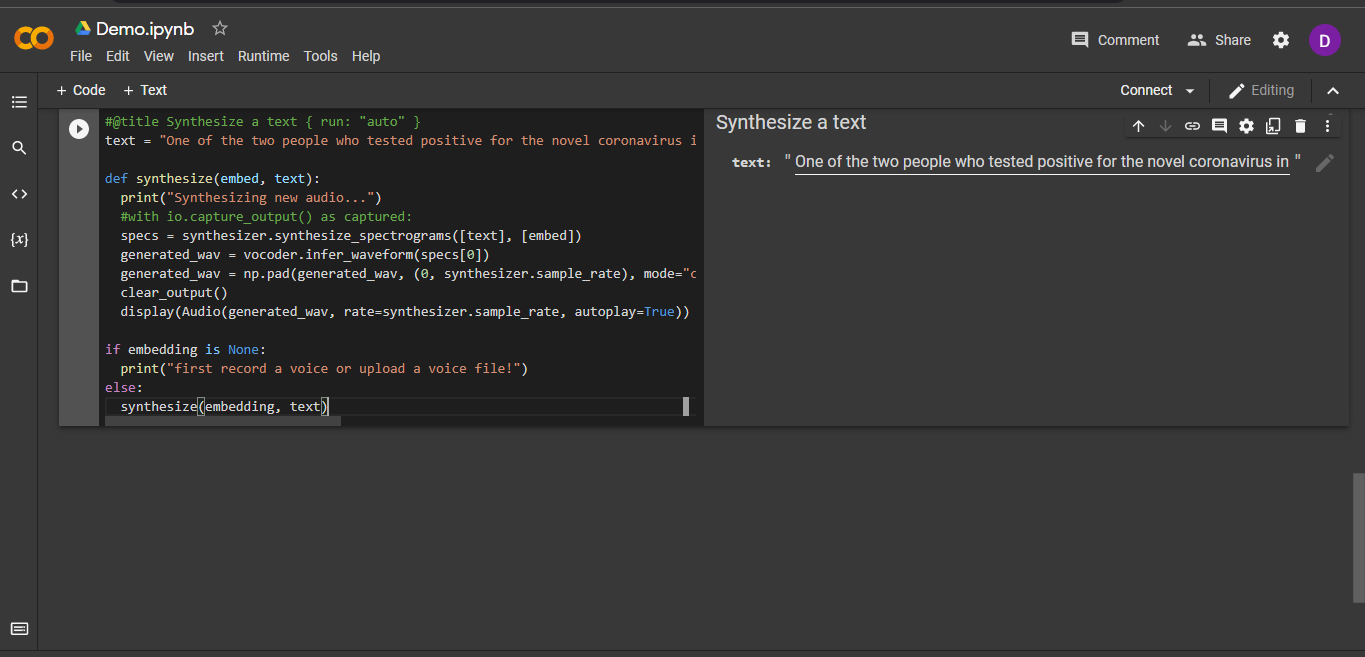
\includegraphics[scale=0.3]{figures/tutor6}
    \caption{\textit{Synthesize and Generate Audio}}
    \label{tutor6}
\end{figure}

\begin{lstlisting}[language=Python, caption=Synthesize dan Generate Audio Output]
#@title Synthesize a text { run: "auto" }
text = "One of the two people who tested positive for the novel coronavirus in the United Kingdom is a student at the University of York in northern England." #@param {type:"string"}
  
def synthesize(embed, text):
  print("Synthesizing new audio...")
  #with io.capture_output() as captured:
  specs = synthesizer.synthesize_spectrograms([text], [embed])
  generated_wav = vocoder.infer_waveform(specs[0])
  generated_wav = np.pad(generated_wav, (0, synthesizer.sample_rate), mode="constant")
  clear_output()
  display(Audio(generated_wav, rate=synthesizer.sample_rate, autoplay=True))

if embedding is None:
  print("first record a voice or upload a voice file!")
else:
  synthesize(embedding, text)
    
\end{lstlisting}
\end{enumerate}

\section{Pembahasan Error dan Solusi}